\newlength{\bibsep}
\documentclass[nonatbib,5p,a4paper]{elsarticle}  % 5p for two columns, 1p for 1 column (this is specific for the elsearticle)
\usepackage[english,norsk,nynorsk]{babel}        % Language
\usepackage[DatePublished]{Code/NTNU-lab}        % remove [DatePublished] to remove dates
\usepackage{csquotes}                            % Must be loaded when babel is loaded to avoid error.
% Use this file to write code that you do not want in the .sty file, but has to be in the preamble (before \begin{document}).
% Writing in this file in stead of in the preamble will keep the main file more organised and tidy.


%                       Nomenclatures
%_______________________________________________________________
\usepackage[intoc]{nomencl}
\makenomenclature

\renewcommand{\nomname}{%
% Title
%----------------
List of Symbols
%----------------
}
\renewcommand{\nompreamble}{%
% Description
%----------------
The next list describes several symbols that will be later used within the body of the document
%----------------
}
% This code creates the groups
\renewcommand\nomgroup[1]{%
  \item[\bfseries
  \ifstrequal{#1}{A}{Physics constants}{%
  \ifstrequal{#1}{B}{Mathematical constants}{%
  \ifstrequal{#1}{C}{Other symbols}{}}}%
]}
% This will add the units
\newcommand{\nomunit}[1]{%
\renewcommand{\nomentryend}{\\#1}}
%................................................................

                            % Write all preamble code in this file to keep it organised and tidy.

% ---------- Additions for the tennis racket report ----------
\usepackage{xcolor,graphicx,booktabs,tabularx}
\usepackage[section]{placeins}                   % keeps each section's floats inside that section
\usetikzlibrary{arrows.meta,positioning}
\newcolumntype{L}{>{\raggedright\arraybackslash}X} % ragged-right X column for wrapping table cells

\newif\ifshowhints
\showhintstrue                                   % \showhintsfalse hides every leftover hint
\definecolor{hintcolor}{RGB}{31,90,180}
% \hint{...}: block telling you what to write here. \hintin{...}: same, inline (use in captions)
\newcommand{\hint}[1]{\ifshowhints\par\noindent{\sloppy\small\sffamily\color{hintcolor}\textbf{[To write]} #1\par}\fi}
\newcommand{\hintin}[1]{\ifshowhints{\color{hintcolor}[#1]}\fi}
% \figslot{file}{what it shows}: shows Images/file if it exists, otherwise a framed placeholder
\newcommand{\figslot}[2]{\IfFileExists{Images/#1}{\includegraphics[width=\linewidth]{Images/#1}}{%
  \fbox{\parbox[c][0.35\linewidth][c]{\dimexpr\linewidth-2\fboxsep-2\fboxrule}{\centering\footnotesize\sffamily\color{gray}%
  \textbf{Images/\detokenize{#1}}\\[2pt]#2}}}}
\newcommand{\code}[1]{\texttt{\detokenize{#1}}}
\appto{\bibsetup}{\sloppy}                         % long titles/URLs in the two-column bibliography
\newcommand{\repourl}{https://github.com/AryanRaval37/tennis-racket-theorem}
% -------------------------------------------------------------

\addbibresource{Bibliography/Sources.bib}        % Selects the Bibliography file.


\begin{document}
\selectlanguage{english}                         % Sets the language of the document.

%%%%%%%%%%%%%%%%%%%%%%%%%%%%%%%%%%%%%%%%

\begin{frontmatter}
%
% Title:
%------------------------------------
\title{%
The Tennis Racket Theorem: A Computational Study of the Intermediate Axis Instability\\
\small Computational Physics (EP4210)
}
%
% Authors:
%------------------------------------
\author{Aryan Raval (EP25BTECH11007)}
\author{Vishal Yalavarti (EP25BTECH11033)}  % TODO roll number
\author{Yug Gandhi (EP25BTECH11035)}        % TODO roll number
%
% Date:
%------------------------------------
\newdate{dateName}{10}{11}{2026}
\renewcommand*{\today}{\DayMonthYearDateFormat\displaydate{dateName}}
%
% Abstract:
%------------------------------------
\NameOfAbstract{Abstract}
\begin{abstract}
The Tennis Racket Theorem also known as the Dzhanibekov effect is when a body rotating close to its interdiate axis (explained below) periodically flips its orientation in space.
Our project involved observing this effect, simulating the rotation of rigid bodies given their initial orientation and angular velocities using two models,
(1) A set of masses connected by rigid springs and (2) Using Quaternions and Euler Equations to store orientation. The first model is basically a simple physics engine that was written in both python and rust
and the second model written in python, is a more direct approach that updates the orientation of the body using rk4 integration. We see that both our models agree as the stiffness of the springs is increased in the first model and the timestep is reduced.
An extension to this project that we explored was adding damping to the springs to observe the fact that a non-rigid body that can loose energy by 'wobbling' will eventually stabilise its rotation to the axis with maximum moment of inertia.
This also explains why the rotation of Earth is stable and why it won't flip upside down.

% \hint{150--250 words, one sentence each:
% (1) what the Dzhanibekov / tennis racket effect is;
% (2) what we simulated: a free rigid body built from point masses joined by stiff springs, integrated with velocity Verlet (Python + Rust engines), plus a direct Euler-equation / quaternion solver;
% (3) headline results: flip only about the middle axis, polhode matches the sphere--ellipsoid intersection, $t_{\text{flip}}\propto\lambda^{-1}\ln(1/\varepsilon)$ with fitted vs predicted $\lambda$, damping drives the body to the max-$I$ axis;
% (4) validation: agreement with the Jacobi elliptic solution, convergence order, energy/$\abs{\vb{L}}$ drift, numbers with errors.}
\end{abstract}
%
\end{frontmatter}
%

\section{Introduction}
\label{sec:intro}

\subsection{A short history of the effect}
\label{sec:history}
The equations governing a rotating rigid body with no torque acting on it were written down by Euler in the 1760s, and in 1834 Poinsot gave the geometric picture of the motion that is still used today: the angular momentum vector rolls along curves on the body's energy ellipsoid \cite{poinsot1834}.
From this analysis it follows that steady rotation about the axes of largest and smallest moment of inertia, the major and minor axes, is stable, while rotation about the intermediate axis is not.

The most famous observation came from space.
In June 1985 the cosmonauts Vladimir Dzha\-ni\-be\-kov and Viktor Savinykh flew Soyuz T-13 to the Salyut 7 space station, which had lost power and stopped responding to ground control months earlier.
They docked manually with the tumbling, frozen station and brought it back to life.
While unpacking supplies, Dzha\-ni\-be\-kov unscrewed a wing nut that spun off the end of its bolt and floated away.
As it drifted across the cabin, the nut flipped by \ang{180} every few seconds, again and again, while its spin stayed otherwise the same.
In microgravity there was nothing to cut the motion short, so the flips repeated periodically, which had never been seen so clearly before.
The phenomenon is now often called the \emph{Dzhanibekov effect} \cite{wiki_trt}.
Popular accounts claim the observation was kept quiet by the Soviet authorities for about a decade and was later linked to speculation that the Earth itself might flip over \cite{veritasium}.
We now know that the Earth won't flip over because it is already spinning about its major axis.

A related lesson had been learned earlier with Explorer 1, the first American satellite, launched in 1958.
It was designed to spin about its long axis, its \emph{minor} axis, but its flexible antennas dissipated energy and within hours it had moved to a tumble about its major axis.
For a body that is not perfectly rigid, only the major axis is truly stable.

The effect is easy to see on Earth.
A tennis racket, a book or a phone tossed in the air while spinning about its intermediate axis comes back having turned over by half a turn about another axis, while spins about the other two axes stay clean.
\begin{figure}[H]
    \centering
    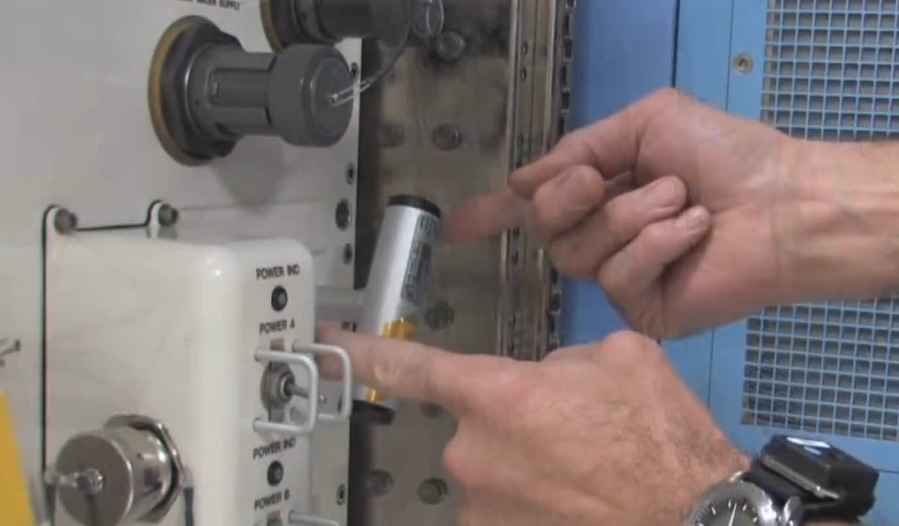
\includegraphics[width=0.6\linewidth]{Images/nasa_demo.jpeg}
    \caption{Demonstration of the effect by NASA astronauts in microgravity \cite{wiki_trt}.}
    \label{fig:intro}
\end{figure}

\makeatletter\if@firstcolumn\null\newpage\fi\makeatother\newpage % Theory starts on a new page (works from either column)

\section{Theory}
\label{sec:theory}

\subsection{Rigid body kinematics}
\label{sec:kinematics}
We describe the body with two frames: a lab frame fixed in space, and a body frame with axes $\vb{e}_1,\vb{e}_2,\vb{e}_3$ that rotate with the body.
The rotation is described by the angular velocity $\vb*{\omega}$, and each body axis moves as $\dot{\vb{e}}_k=\vb*{\omega}\times\vb{e}_k$.
We write $\Omega_k=\vb*{\omega}\vdot\vb{e}_k$ for the components of $\vb*{\omega}$ in the body frame.
For a free body no torque acts, so the angular momentum $\vb{L}$ is fixed in the lab frame.
Seen from the body, however, $\vb{L}$ moves, and following this motion is the key to the effect.

\subsection{The inertia tensor}
\label{sec:inertia}
For a body made of point masses $m_i$ at positions $\vb{r}_i$ from the centre of mass, the inertia tensor is
\begin{equation}
    I_{ab} = \sum_i m_i\left(r_i^2\,\delta_{ab} - r_{i,a}\,r_{i,b}\right)
    \label{eq:inertia}
\end{equation}
and $\vb{L}=\mathsf{I}\,\vb*{\omega}$.
In general $\vb{L}$ and $\vb*{\omega}$ are not parallel.
Since $\mathsf{I}$ is symmetric, there are three perpendicular \emph{principal axes} in which it is diagonal, with principal moments $I_1>I_2>I_3$.
Spinning about any one of them keeps $\vb{L}$ parallel to $\vb*{\omega}$.
Our main body is an octahedron of six \SI{1}{kg} masses at $(\pm1,0,0)$, $(0,\pm2,0)$ and $(0,0,\pm3)$\,m, whose principal axes are $x$, $y$ and $z$ with $I_x=26$, $I_y=20$ and $I_z=\SI{10}{kg.m^2}$, so $y$ is the middle axis.

\subsection{Euler's equations}
\label{sec:euler}
Written in the body frame along the principal axes, $\dot{\vb{L}}=0$ becomes Euler's equations,
\begin{equation}
\begin{aligned}
    I_1\dot\Omega_1 &= (I_2 - I_3)\,\Omega_2\Omega_3\\
    I_2\dot\Omega_2 &= (I_3 - I_1)\,\Omega_3\Omega_1\\
    I_3\dot\Omega_3 &= (I_1 - I_2)\,\Omega_1\Omega_2
\end{aligned}
\label{eq:euler}
\end{equation}
They conserve the kinetic energy and the magnitude of the angular momentum,
\begin{equation}
    2E = \sum_k \frac{L_k^2}{I_k},\qquad L^2 = \sum_k L_k^2,
    \label{eq:conserved}
\end{equation}
with $L_k=I_k\Omega_k$.
These two quantities are what we monitor to check our simulations (\cref{sec:conservation}).

\subsection{Instability of the middle axis}
\label{sec:stability}
Suppose the body spins with rate $\Omega$ about one principal axis and is given a small tilt.
It can be shown that about the axes of largest and smallest moment the tilt only oscillates, but about the intermediate axis it grows as $e^{\lambda t}$ with
\begin{equation}
    \lambda = \Omega\sqrt{\frac{(I_1-I_2)(I_2-I_3)}{I_1 I_3}}.
    \label{eq:lambda}
\end{equation}
For the octahedron this gives $\lambda\approx0.480\,\Omega$.
If the initial tilt has size $\varepsilon$, it becomes of order one, which is a flip, after roughly
\begin{equation}
    t_{\text{flip}} \approx \frac{1}{\lambda}\ln\frac{1}{\varepsilon},
    \label{eq:tflip}
\end{equation}
so the flip time grows only slowly as the tilt is made smaller.
We test this in \cref{sec:res-fliptime}.

\subsection{Geometric picture: the polhode}
\label{sec:polhode}
\Cref{eq:conserved} gives a simple picture of the motion.
In the body frame $\vb{L}$ must lie on a sphere of radius $L$ and, at the same time, on the energy ellipsoid.
It therefore moves along the curve where the two surfaces meet, called the polhode (\cref{fig:polhode-family}).
Near the largest and smallest axes these curves are small closed loops, so $\vb{L}$ stays close to the axis and the rotation is stable.
Near the middle axis the two surfaces cross, and the special curve through this axis, the separatrix, carries $\vb{L}$ all the way to the opposite side.
\begin{figure}[H]
    \centering
    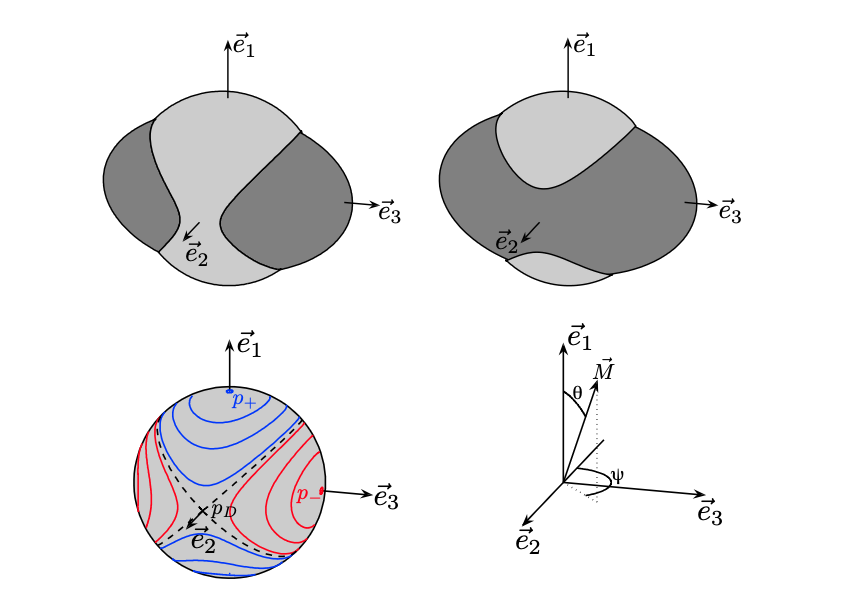
\includegraphics[width=\linewidth]{Images/polhode_vandamme.png}
    \caption{Top: the energy ellipsoid (dark) and the angular momentum sphere (light). Bottom left: polhodes on the sphere, with the separatrix dashed. Adapted from \cite{vandamme2017}.}
    \label{fig:polhode-family}
\end{figure}

\makeatletter\if@firstcolumn\null\newpage\fi\makeatother\newpage % Method starts on a new page
\section{Method}
\label{sec:methods}

\subsection{Overview of the pipeline}
\Cref{fig:pipeline} shows how the parts of the project fit together.
Both solvers start from an initial spin and write their results to CSV files, and the analysis and animation scripts work from these files.
\begin{figure}[htb]
    \centering
    \begin{tikzpicture}[node distance=0.5cm and 0.6cm,
        box/.style={draw,rounded corners=2pt,align=center,font=\scriptsize\sffamily,minimum height=0.9cm,text width=2.1cm},
        arr/.style={-{Stealth[length=1.8mm]},thick}]
        \node[box] (ic) {Initial spin\\ $\vb*{\omega}_0$};
        \node[box,right=of ic] (eng) {Spring-mass engine\\ Python / Rust, Verlet};
        \node[box,below=of ic] (rb) {Rigid-body solver\\ Euler eqs.\ + quaternions, RK4};
        \node[box,below=of eng] (csv) {CSV files};
        \node[box,below=of csv] (ana) {Analysis\\ NumPy / SciPy};
        \node[box,left=of ana] (out) {Plots \&\\ Manim videos};
        \draw[arr] (ic) -- (eng); \draw[arr] (eng) -- (csv); \draw[arr] (csv) -- (ana);
        \draw[arr] (ic) -- (rb); \draw[arr] (rb) -- (csv); \draw[arr] (ana) -- (out);
    \end{tikzpicture}
    \caption{Overview of the simulation and analysis pipeline. The spring engines start from $\vb{v}_i=\vb*{\omega}_0\times\vb{r}_i$, the rigid-body solver from $\vb*{\Omega}_0=\vb*{\omega}_0$ and $q_0=(1,\vb{0})$.}
    \label{fig:pipeline}
\end{figure}

\subsection{The rigid body as point masses and springs}
\label{sec:spring-model}
In our first approach no rigid body equations are coded at all.
The body is built from a few point masses, and every pair of masses is joined by a stiff spring whose rest length is the initial distance between them (\code{rigid=True} in \code{System}).
With $N$ masses there are $N(N-1)/2$ springs, so the six-mass octahedron has 15.
Each spring pulls along the line joining its two masses, with a force proportional to its stretch plus an optional damping term proportional to the rate of stretching (\cref{lst:spring}).
These forces are equal, opposite and central, so the total momentum and angular momentum are conserved, and damping only removes energy.
Rigid body motion, Euler's equations and the flip are not put in by hand; they have to emerge from Newton's second law for the individual masses.

\medskip\noindent\begin{minipage}{\linewidth}
\begin{minted}[bgcolor=LightGray,breaklines,fontsize=\scriptsize]{python}
def _spring_force(self, x, v, t):
    F = np.zeros_like(x)
    for (i, j, k, c, rest) in self.springs:
        d = x[j] - x[i]  # points from i to j
        r = np.linalg.norm(d)
        s = k*(r - rest) + c*np.dot(v[j] - v[i], d)/r
        f = s*d/r
        F[i] += f
        F[j] -= f
    return F
\end{minted}
\captionof{listing}{Spring forces on all masses (\code{engine.py}, condensed).}
\label{lst:spring}
\end{minipage}\par\medskip

The springs have to be stiff so that the body barely deforms.
With $k=\SI{e5}{N/m}$ and \SI{1}{kg} masses they vibrate at $\omega_s\sim\sqrt{k/m}\approx\SI{300}{rad/s}$, while the body itself turns at about \SI{1}{rad/s}.
The time step has to resolve these fast vibrations, which makes the model expensive.
For this reason the engine, first written in Python, was ported with the same structure to Rust for the long runs with small time steps.

\subsubsection{Velocity Verlet}
\label{sec:verlet}
Newton's equations for the masses are integrated with the velocity Verlet scheme in its kick--drift--kick form,
\begin{equation}
\begin{aligned}
    \vb{v}_i^{n+1/2} &= \vb{v}_i^{n} + \tfrac{\Delta t}{2m_i}\vb{F}_i(\vb{x}^{n})\\
    \vb{x}_i^{n+1}   &= \vb{x}_i^{n} + \Delta t\,\vb{v}_i^{n+1/2}\\
    \vb{v}_i^{n+1}   &= \vb{v}_i^{n+1/2} + \tfrac{\Delta t}{2m_i}\vb{F}_i(\vb{x}^{n+1})
\end{aligned}
\label{eq:verlet}
\end{equation}
Each mass gets half a velocity kick from the current forces, moves for a full step, and gets the second half kick from the forces at its new position.
The forces from the end of one step are reused at the start of the next, so only one force evaluation is needed per step (\cref{lst:verlet}).
Verlet is second order, time-reversible and symplectic, so the energy error stays bounded over long runs instead of drifting \cite{verlet1967,hairer2006}.
This is the very reason we chose to use this over RK4, which is more accurate over one step.

\medskip\noindent\begin{minipage}{\linewidth}
\begin{minted}[bgcolor=LightGray,breaklines,fontsize=\scriptsize]{python}
def step(self, dt):
    self.v += 0.5*dt*self.force_cached/self.m  # half kick
    self.x += dt*self.v                         # drift
    self.t += dt
    self.force_cached = self.total_force()
    self.v += 0.5*dt*self.force_cached/self.m  # half kick
\end{minted}
\captionof{listing}{One velocity Verlet step (\code{engine.py}; \code{RigidBody::step} in Rust is the same).}
\label{lst:verlet}
\end{minipage}\par\medskip

\subsection{Direct rigid body solver with quaternions}
\label{sec:quaternions}
While the spring model is general, it is indirect and expensive: the body is only approximately rigid, and the stiff springs force a tiny time step.
A truly rigid body needs much less information.
Its state is just its angular velocity and its orientation, and nothing in it vibrates, so the time step only has to resolve the rotation itself.
As an independent check we therefore also solve the rigid body equations directly (\code{quaternion.py}).
The angular velocity $\vb*{\Omega}$ in the body frame follows Euler's equations (\cref{eq:euler}).
The remaining question is how to store the orientation.

\paragraph{Choosing a representation}
Three Euler angles are the most familiar choice and use the minimum number of variables, but their equations of motion contain $1/\sin\theta$ and blow up when two rotation axes line up (this is called gimbal lock), and every step needs trigonometric functions.
A $3\times3$ rotation matrix has to store nine numbers for three degrees of freedom; numerical errors slowly make it non-orthogonal, so it stops being a pure rotation and has to be re-orthogonalised.
We found that there is a very beautiful way of describing these rotations using quaternions \cite{3b1b_quat}. These are complex numbers but in 4D.
A rotation by an angle $\phi$ about a unit axis $\vu{n}$ is written as
\begin{equation}
    q = \left(\cos\tfrac{\phi}{2},\ \vu{n}\sin\tfrac{\phi}{2}\right), \qquad \abs{q}=1,
    \label{eq:quat-def}
\end{equation}
a scalar and a vector part, and two quaternions are multiplied as
\begin{equation}
\begin{aligned}
    (a,\vb{a})\otimes(b,\vb{b}) = \big(&ab-\vb{a}\vdot\vb{b},\\
                                       &a\vb{b}+b\vb{a}+\vb{a}\times\vb{b}\big).
\end{aligned}
    \label{eq:quat-mult}
\end{equation}
Combining two rotations is a single product, with 16 multiplications instead of the 27 of a matrix product.

\paragraph{Equations of motion}
With this representation the orientation evolves as
\begin{equation}
    \dot q = \tfrac12\, q\otimes(0,\vb*{\Omega}),\qquad
    \vb{r}_{\text{lab}} = q\otimes(0,\vb{r}_{\text{body}})\otimes q^{*}.
    \label{eq:quat}
\end{equation}
The first equation is linear in $q$ and contains only products and sums, with no trigonometric functions and no singular points, which makes it both cheap and robust to integrate.
The only constraint is $\abs{q}=1$, which numerical errors break slowly and which is restored by simply dividing $q$ by its length.
The second relation rotates any point of the body into the lab frame, which we use for plots and animations.
In total the state is seven numbers, $\vb*{\Omega}$ and $q$, and \cref{eq:euler,eq:quat} are solved together (\cref{lst:derivs}).

\begin{sloppypar} % units and reference names would otherwise stick out of the column
\paragraph{The racket}
We use this solver for a real racket, the Babolat Pure Drive 2025, with the specifications listed by Tennis Warehouse \cite{tw_puredrive,twu_analyzer}: mass \SI{318}{g} strung, balance point \SI{32.99}{cm} from the butt, swingweight \SI{317}{kg.cm^2} and twistweight \SI{15.7}{kg.cm^2}.
For the racket we number the axes from the handle (1, smallest moment) to the face normal (3, largest), the reverse of \cref{sec:inertia}; Euler's equations (\cref{eq:euler}) hold in any right-handed principal frame, and \cref{eq:lambda} is unchanged when $I_1$ and $I_3$ are swapped.
The twistweight is the moment about the handle, $I_1=\SI{1.57e-3}{kg.m^2}$.
The swingweight is measured about an axis \SI{10}{cm} from the butt, so the parallel-axis theorem gives $I_2=\SI{1.49e-2}{kg.m^2}$ about the centre of mass, and because the racket is nearly flat the perpendicular-axis theorem gives $I_3=I_1+I_2=\SI{1.65e-2}{kg.m^2}$.
The racket is thrown with $\vb*{\Omega}_0=(-1.96,\,9.26,\,0)\,\si{rad/s}$, chosen so that after the \SI{0.7}{s} flight it has made exactly half a turn about its handle.
\end{sloppypar}

\medskip\noindent\begin{minipage}{\linewidth}
\begin{minted}[bgcolor=LightGray,breaklines,fontsize=\scriptsize]{python}
def euler_equations(w):
    w1, w2, w3 = w
    return np.array([(I2 - I3)/I1*w2*w3,
                     (I3 - I1)/I2*w3*w1,
                     (I1 - I2)/I3*w1*w2])

def dq(q, w):
    return 0.5*quaternion_multiply(q, [0, *w])
\end{minted}
\captionof{listing}{Time derivatives of $\vb*{\Omega}$ and $q$ (\code{quaternion.py}, condensed).}
\label{lst:derivs}
\end{minipage}\par\medskip

\subsubsection{Fourth-order Runge--Kutta}
\label{sec:rk4}
This system has no stiff springs, so we integrate it with the fourth-order Runge--Kutta method (RK4),
\begin{equation}
    \vb{y}_{n+1} = \vb{y}_n + \frac{\Delta t}{6}\left(\vb{k}_1+2\vb{k}_2+2\vb{k}_3+\vb{k}_4\right),
    \label{eq:rk4}
\end{equation}
with $\vb{y}=(\vb*{\Omega},q)$ and $\Delta t=\SI{1}{ms}$.
$\vb*{\Omega}$ and $q$ are advanced together, so each of the four stages evaluates both derivatives (\cref{lst:rk4}).
RK4 does not keep $\abs{q}=1$ exactly, so $q$ is renormalised after every step.

\medskip\noindent\begin{minipage}{\linewidth}
\begin{minted}[bgcolor=LightGray,breaklines,fontsize=\scriptsize]{python}
def rk4(w, q, dt):
    k1, l1 = euler_equations(w), dq(q, w)
    w2 = w + 0.5*dt*k1
    k2, l2 = euler_equations(w2), dq(q + 0.5*dt*l1, w2)
    w3 = w + 0.5*dt*k2
    k3, l3 = euler_equations(w3), dq(q + 0.5*dt*l2, w3)
    w4 = w + dt*k3
    k4, l4 = euler_equations(w4), dq(q + dt*l3, w4)
    w = w + dt/6*(k1 + 2*k2 + 2*k3 + k4)
    q = q + dt/6*(l1 + 2*l2 + 2*l3 + l4)
    return w, q/np.linalg.norm(q)  # keep |q| = 1
\end{minted}
\captionof{listing}{One RK4 step for $\vb*{\Omega}$ and $q$ (\code{quaternion.py}, condensed).}
\label{lst:rk4}
\end{minipage}\par\medskip

\subsection{Observables from particle positions}
\label{sec:observables}
The spring engines only save the positions of the masses, 60 times per simulated second.
Everything else is computed from these positions afterwards (\code{src/sim/}); only the conservation checks of \cref{sec:conservation} use the engine's own velocities.
\begin{sloppypar} % long words would otherwise stick out of the column
\begin{itemize}
    \item \textbf{Body axes.} The masses sit in opposite pairs on the principal axes, so the unit vector from one mass of a pair to the other gives that body axis $\vb{e}_k$.
    \item \textbf{Velocities.} Computed with \code{np.gradient}, which takes second-order finite differences of the saved positions.
    \item \textbf{Angular velocity.} Each axis moves as $\dot{\vb{e}}_k=\vb*{\omega}\times\vb{e}_k$; summing $\vb{e}_k\times\dot{\vb{e}}_k$ over the three axes gives $2\vb*{\omega}$, so
    \begin{equation}
        \vb*{\omega} = \frac12\sum_{k=1}^{3}\vb{e}_k\times\dot{\vb{e}}_k,
        \qquad \Omega_k = \vb*{\omega}\vdot\vb{e}_k.
        \label{eq:omega-from-axes}
    \end{equation}
    \item \textbf{Angular momentum.} $\vb{L}=\sum_i m_i\,\vb{r}_i\times\vb{v}_i$ about the centre of mass, projected onto the body axes to draw the polhode.
    \item \textbf{Flips.} A flip is counted each time the component of $\vb{L}$ along the intermediate axis changes sign.
\end{itemize}
\end{sloppypar}
For the quaternion solver $\vb*{\Omega}$ and $q$ are the state itself, so nothing has to be reconstructed.

\subsection{Implementation}
\label{sec:implementation}
\begin{sloppypar} % long code names would otherwise stick out of the column
The spring engine was first written in Python (\code{engine.py}) and then rewritten in Rust with the same design.
Both are small general-purpose engines: they know nothing about rigid bodies or Euler's equations, only about point masses and the forces between them.

\paragraph{Python engine}
A \code{System} object stores the positions, velocities and masses of all particles as NumPy arrays.
Masses are added with \code{add_mass}, springs with \code{add_spring}, and any other force (for example gravity or an external torque) with \code{add_force}, as a function that takes the current positions, velocities and time and returns the force on every mass.
With \code{rigid=True} the system joins every pair of masses with a spring before the first step.
At each step the forces from all these sources are summed and passed to the Verlet integrator (\cref{lst:verlet}), so adding new physics never requires touching the integrator.
The loop over springs runs in interpreted Python, which makes runs with $\Delta t=\SI{e-5}{s}$ ($10^7$ steps) impractically slow.
\end{sloppypar}

\paragraph{Rust engine}
The Rust version is a library split into small modules (\cref{lst:tree}).
\code{Vector3} is a plain 3D vector with overloaded arithmetic, dot and cross products, so the physics code reads like the equations.
A \code{RigidBody} owns its masses, springs and external forces, and its \code{step} is the same Verlet step as in Python.
An \code{Engine} holds one or more bodies and the clock, and each experiment is a short program in \code{examples/} that builds a body and runs it (\cref{lst:usage}).
Being compiled, the Rust engine is about 500 times faster than the Python one on the same run (\cref{tab:performance}): a $10^7$-step run takes under a second instead of seven minutes.

\medskip\noindent\begin{minipage}{\linewidth}
\begin{minted}[bgcolor=LightGray,breaklines,fontsize=\scriptsize]{text}
src/
  math/vector3.rs     Vector3 and its operators
  body/mass.rs        Mass {m, x, v}
  body/rigid_body.rs  springs, forces, Verlet step
  physics/spring.rs   damped spring force
  physics/force.rs    external force closures
  engine.rs           bodies, clock, CSV export
examples/             one program per run
\end{minted}
\captionof{listing}{Structure of the Rust engine (\code{physics-engine-rs}).}
\label{lst:tree}
\end{minipage}\par\medskip

\medskip\noindent\begin{minipage}{\linewidth}
\begin{minted}[bgcolor=LightGray,breaklines,fontsize=\scriptsize]{rust}
let mut b = RigidBody::new(true, 1e5, 0.0); // rigid, k, c
for r in positions {
    b.add_mass(m, r, w.cross(&r)); // v = w x r
}
let mut u = Engine::new();
u.add_body(b);
u.export_csv("six_masses_rs.csv", 1e-5, 60.0, 100.0)?;
\end{minted}
\captionof{listing}{Setting up and running a simulation with the Rust engine (condensed from \code{examples/}).}
\label{lst:usage}
\end{minipage}\par\medskip

\paragraph{Output and analysis}
Both engines write the same CSV format: a short header with $\Delta t$, the output rate, the masses and the list of springs, followed by one row per frame with the time and all positions.
The animation scripts in \code{src/sim/} therefore work with either engine.
They compute the observables of \cref{sec:observables} with NumPy \cite{numpy} and produce the Manim animations \cite{manim}.
We used AI tools to write the code that creates the videos and the code that exports the CSV files in this format after the runs.
Every other piece of code in the Python and Rust engines and the quaternion file is handwritten. We could not have made the beautiful videos demonstrating this effect without AI and consider this as fair use.


\begin{table}[htb]
    \centering
    \caption{Wall-clock time to integrate the octahedron for $T=\SI{100}{s}$ with $k=\SI{e5}{N/m}$, same initial state. After $10^5$ steps both engines end with bit-for-bit identical positions and velocities.}
    \label{tab:performance}
    \small
    \begin{tabular}{@{}lccc@{}}
        \toprule
        $\Delta t$ (s) & Steps & Python (s) & Rust (s) \\
        \midrule
        $10^{-3}$ & $10^5$ & 4.3 & 0.01 \\
        $10^{-5}$ & $10^7$ & 429 & 0.73 \\
        \bottomrule
    \end{tabular}
\end{table}
This shows how terribly slow Python is for computation whenever loops are involved.

\section{Visualisation}
\label{sec:visualisation}
Every run is turned into an animation with Manim \cite{manim} (\code{src/sim/draw*.py}).
Each video shows the moving body next to live plots of the quantities from \cref{sec:observables}, so the motion and the numbers can be followed together.
The full videos are listed in \ref{app:videos}; this section shows stills from them.

Each script reads a CSV file written by one of the engines, rebuilds the body from the masses and springs listed in its header, and computes the body axes, $\vb*{\Omega}$ and $\vb{L}$ frame by frame as in \cref{sec:observables}.
The playback speed is chosen so that the motion is easy to follow: the octahedron runs are sped up four times, the long damped run twelve times, and the \SI{0.7}{s} racket toss is shown in slow motion.
The videos are rendered at $3840\times2160$ pixels and 60 frames per second.
Seeing the body and the plots side by side also served as a quick check of the simulations, for example that $\vb{L}$ really stays fixed in space while the body turns over.

\Cref{fig:vis-omega,fig:vis-polhode} follow the octahedron spun about its intermediate axis, the first as a still from the video and the second as a plot of $\vb{L}$ seen from the body, made from the same data.
\Cref{fig:vis-racket} shows one toss of a tennis racket computed with the quaternion solver, and \cref{fig:vis-major} shows a damped body moving to its major axis.

\begin{figure*}[tp]
    \centering
    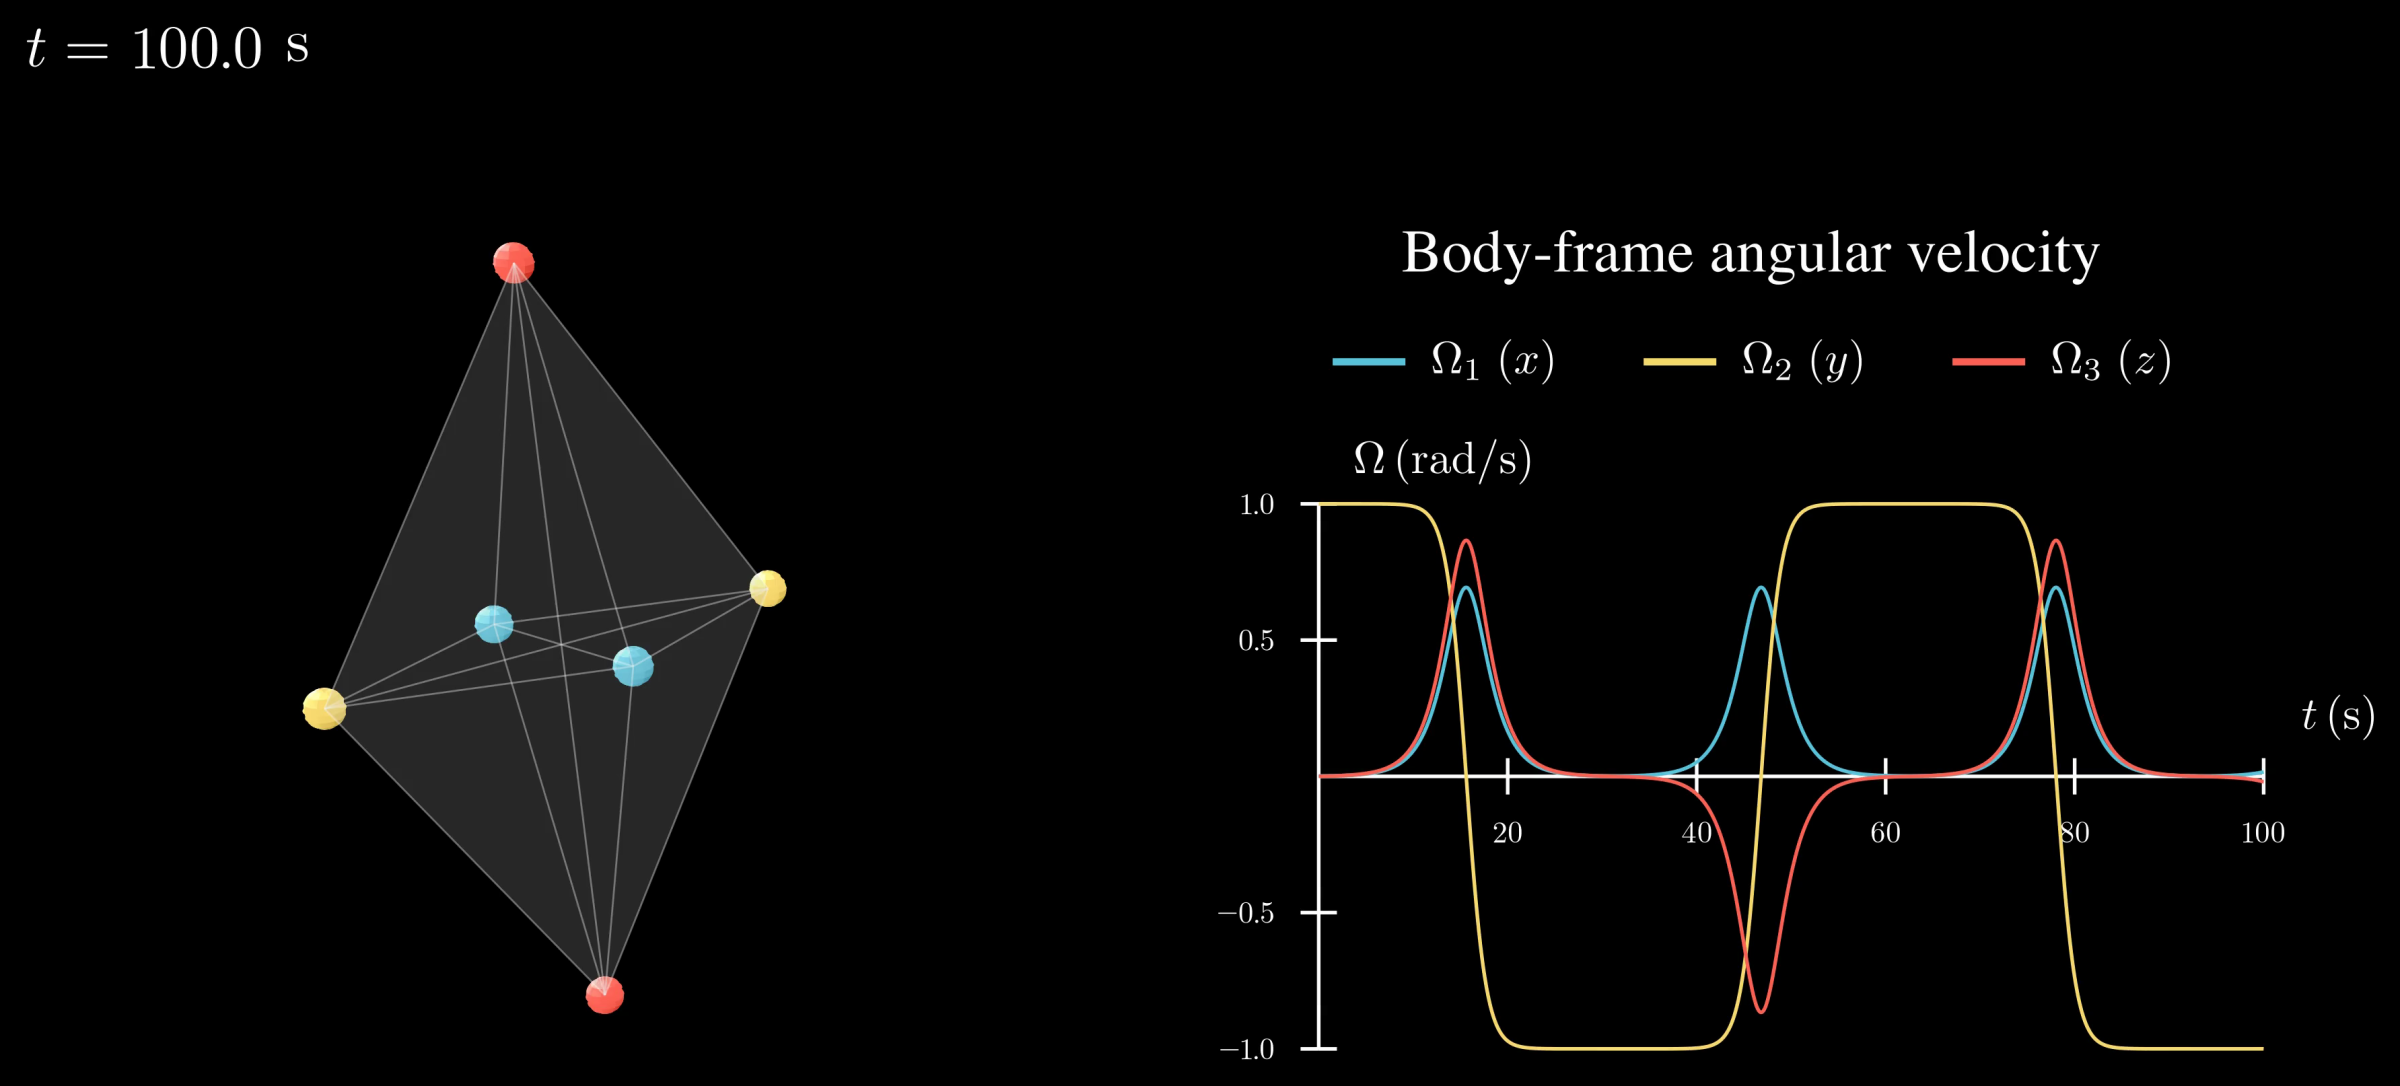
\includegraphics[width=0.9\textwidth]{Images/vis_omega.png}
    \caption{Octahedron (\cref{sec:inertia}) spun at \SI{1}{rad/s} about its intermediate axis $y$ (spring engine, $t=0$--\SI{100}{s}). Left: the body at the end of the run. Right: the body-frame angular velocity. $\Omega_2$ stays almost constant for long stretches and then suddenly reverses sign; each reversal is a flip. During a flip the spin briefly moves into the other two axes, giving the pulses in $\Omega_1$ and $\Omega_3$. The flips repeat regularly, here three times in \SI{100}{s}.}
    \label{fig:vis-omega}
\end{figure*}

\begin{figure*}[tp]
    \centering
    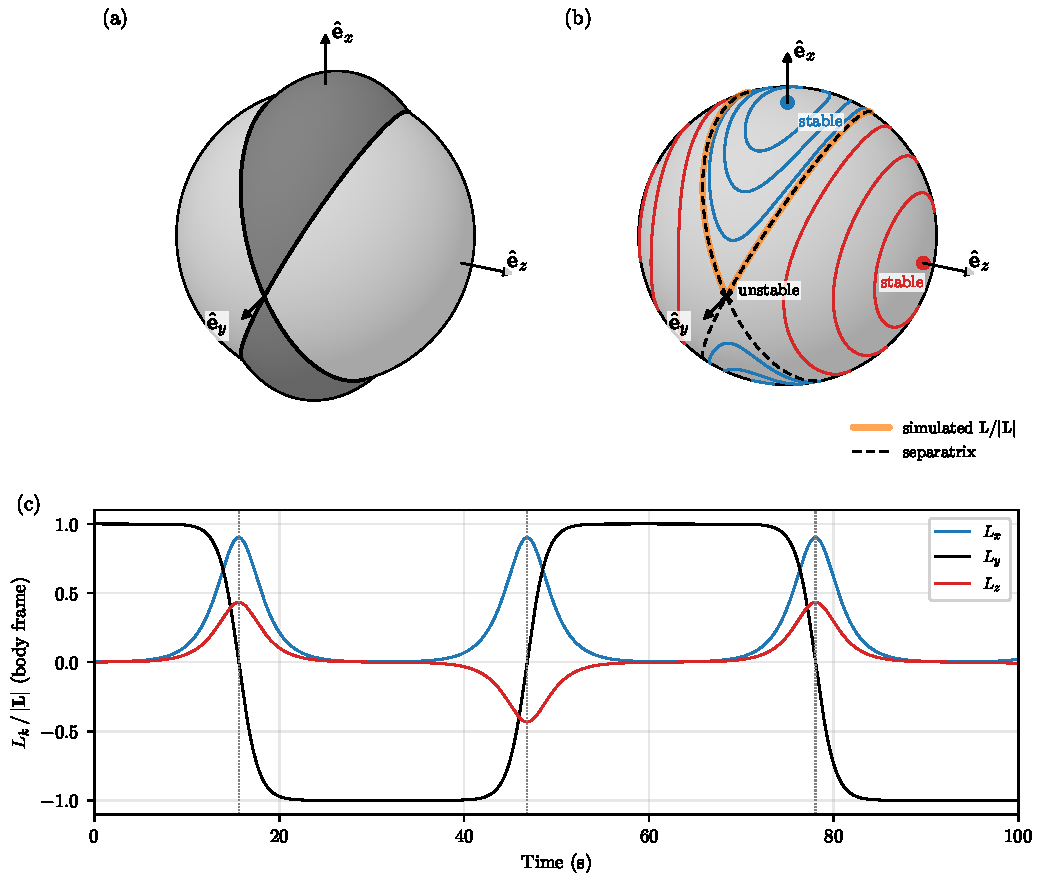
\includegraphics[width=0.75\textwidth]{Images/polhode_sim.pdf}
    \caption{Angular momentum in the body frame for the same run, plotted from the simulation data. (a) The energy ellipsoid of this run (dark grey) cuts the sphere $\abs{\vb{L}}=\text{const}$ (light grey); $\vb{L}$ must stay on the curves where they meet, which here lie almost on the separatrix through the intermediate axis $\vu{e}_y$. (b) Polhodes at other energies: blue curves circle the stable major axis $\vu{e}_x$, red curves the stable minor axis $\vu{e}_z$, and the dashed separatrix crosses at the unstable intermediate axis. The simulated $\vb{L}/\abs{\vb{L}}$ over the whole \SI{100}{s} (orange) runs just beside the separatrix, too close to tell apart here (\cref{sec:analytic}); $2E/L^2$ changes by less than $10^{-5}$ of its value. (c) Body-frame components of $\vb{L}$: $L_y$ jumps between $\pm1$ at each flip (dotted lines, every \SI{31.2}{s}), while $\vb{L}$ passes through the $x$ side of the sphere.}
    \label{fig:vis-polhode}
\end{figure*}

\begin{figure*}[tp]
    \centering
    \begin{minipage}[c]{0.48\textwidth}\centering
        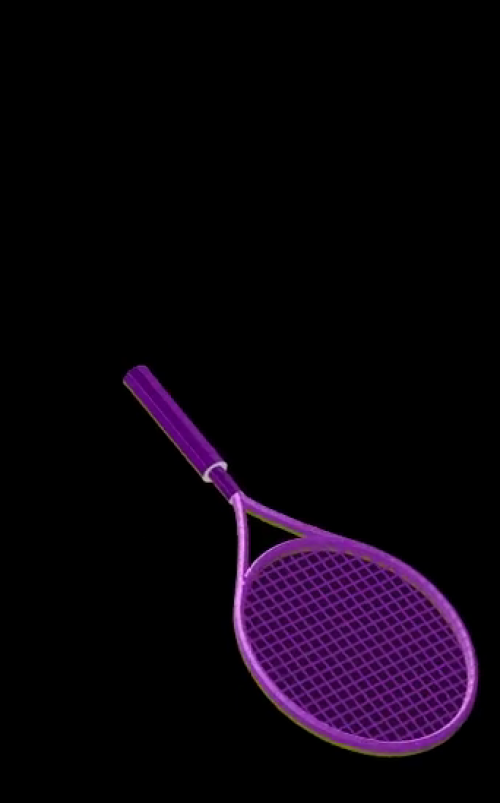
\includegraphics[width=0.32\linewidth]{Images/vis_racket_1.png}\hfill
        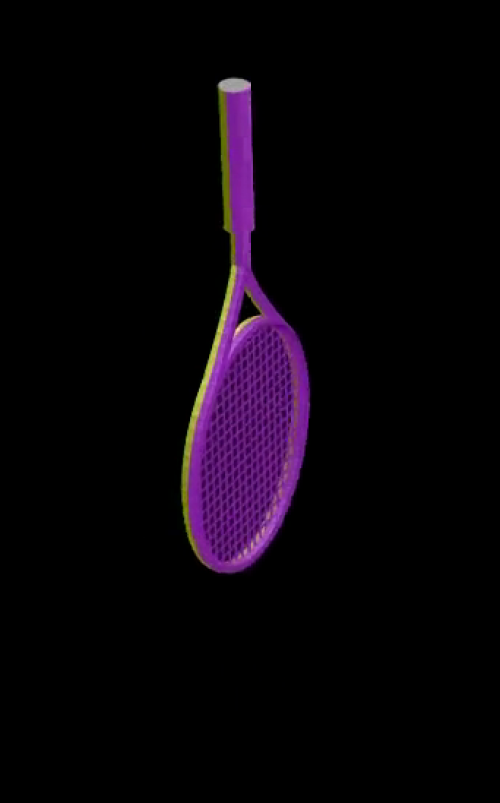
\includegraphics[width=0.32\linewidth]{Images/vis_racket_2.png}\hfill
        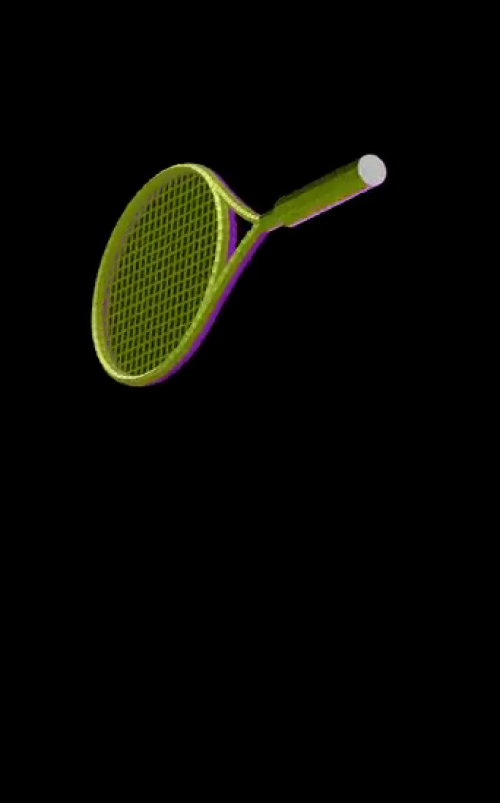
\includegraphics[width=0.32\linewidth]{Images/vis_racket_3.png}\\
        {\footnotesize \makebox[0.32\linewidth]{$t=\SI{0.04}{s}$}\hfill\makebox[0.32\linewidth]{$\SI{0.18}{s}$}\hfill\makebox[0.32\linewidth]{$\SI{0.28}{s}$}}\\[4pt]
        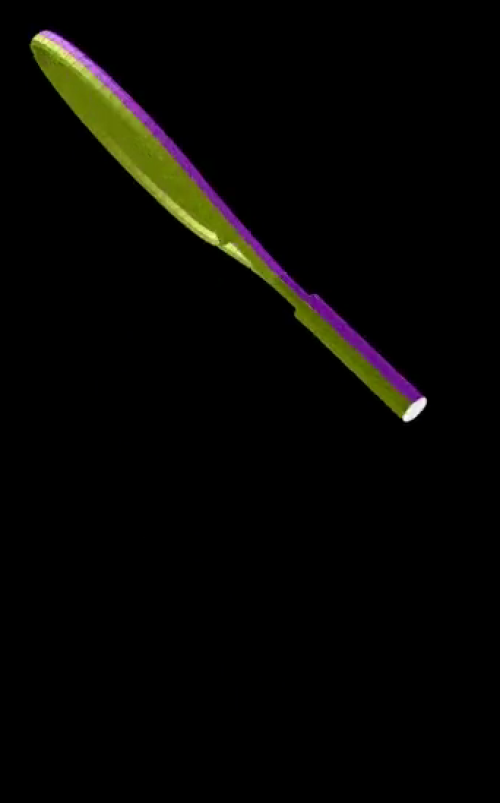
\includegraphics[width=0.32\linewidth]{Images/vis_racket_4.png}\hfill
        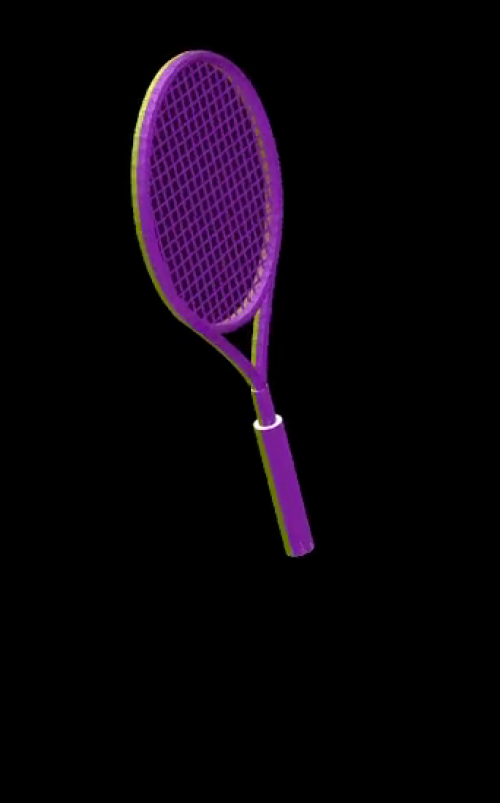
\includegraphics[width=0.32\linewidth]{Images/vis_racket_5.png}\hfill
        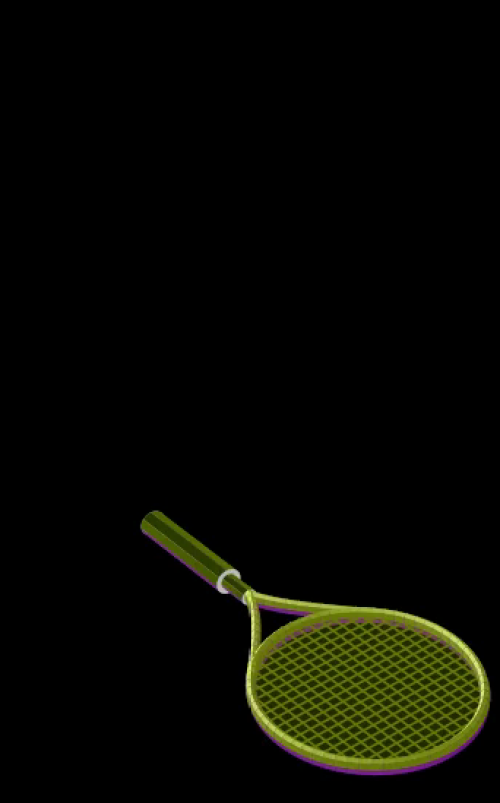
\includegraphics[width=0.32\linewidth]{Images/vis_racket_6.png}\\
        {\footnotesize \makebox[0.32\linewidth]{$\SI{0.40}{s}$}\hfill\makebox[0.32\linewidth]{$\SI{0.52}{s}$}\hfill\makebox[0.32\linewidth]{$\SI{0.70}{s}$}}
    \end{minipage}\hfill
    \begin{minipage}[c]{0.48\textwidth}\centering
        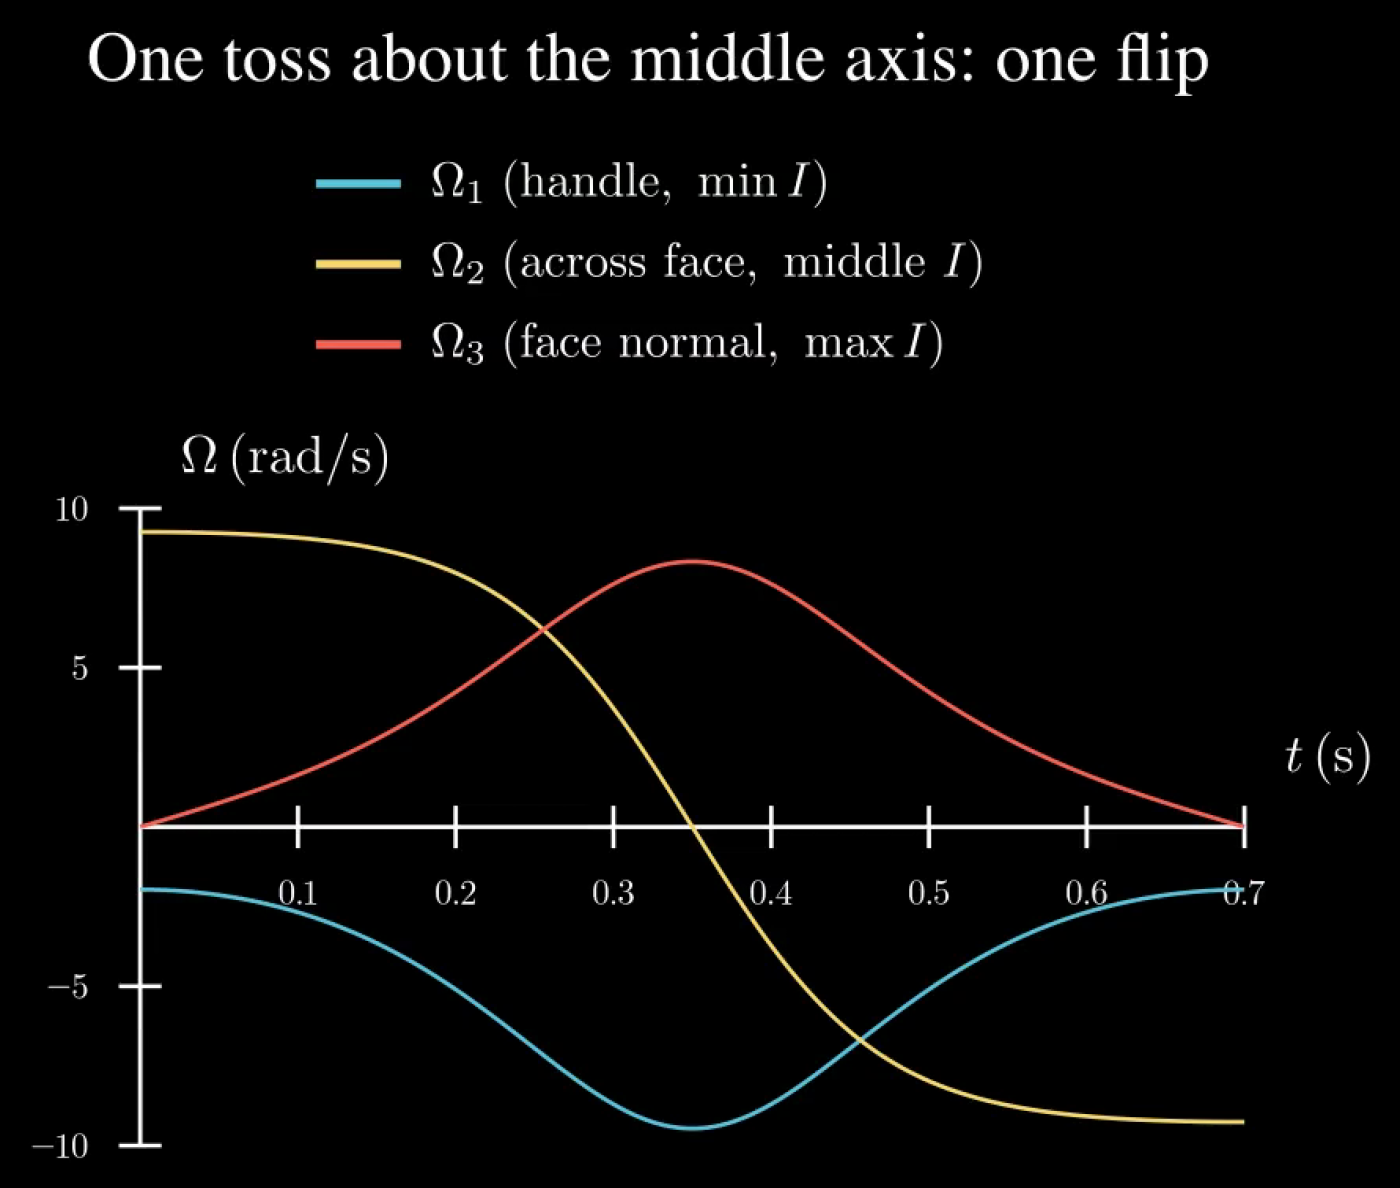
\includegraphics[width=\linewidth]{Images/vis_racket_plot.png}
    \end{minipage}
    \caption{One toss of a tennis racket (\code{quaternion.py}, RK4 with quaternions). The racket is thrown spinning end over end, about its intermediate axis, with a twist about the handle of 21\% of the main spin, which tilts $\vb{L}$ only \ang{1.3} from the intermediate axis. The two sides of the strings are drawn in different colours (purple and yellow). Left: snapshots during the \SI{0.7}{s} flight; the racket comes back with the other side of the face showing, having made a half turn about its handle. Right: the body-frame angular velocity. As $\Omega_2$ (intermediate axis) reverses, the spin passes through the handle ($\Omega_1$) and face-normal ($\Omega_3$) axes, the same pattern as one flip in \cref{fig:vis-omega}.}
    \label{fig:vis-racket}
\end{figure*}

\begin{figure*}[tp]
    \centering
    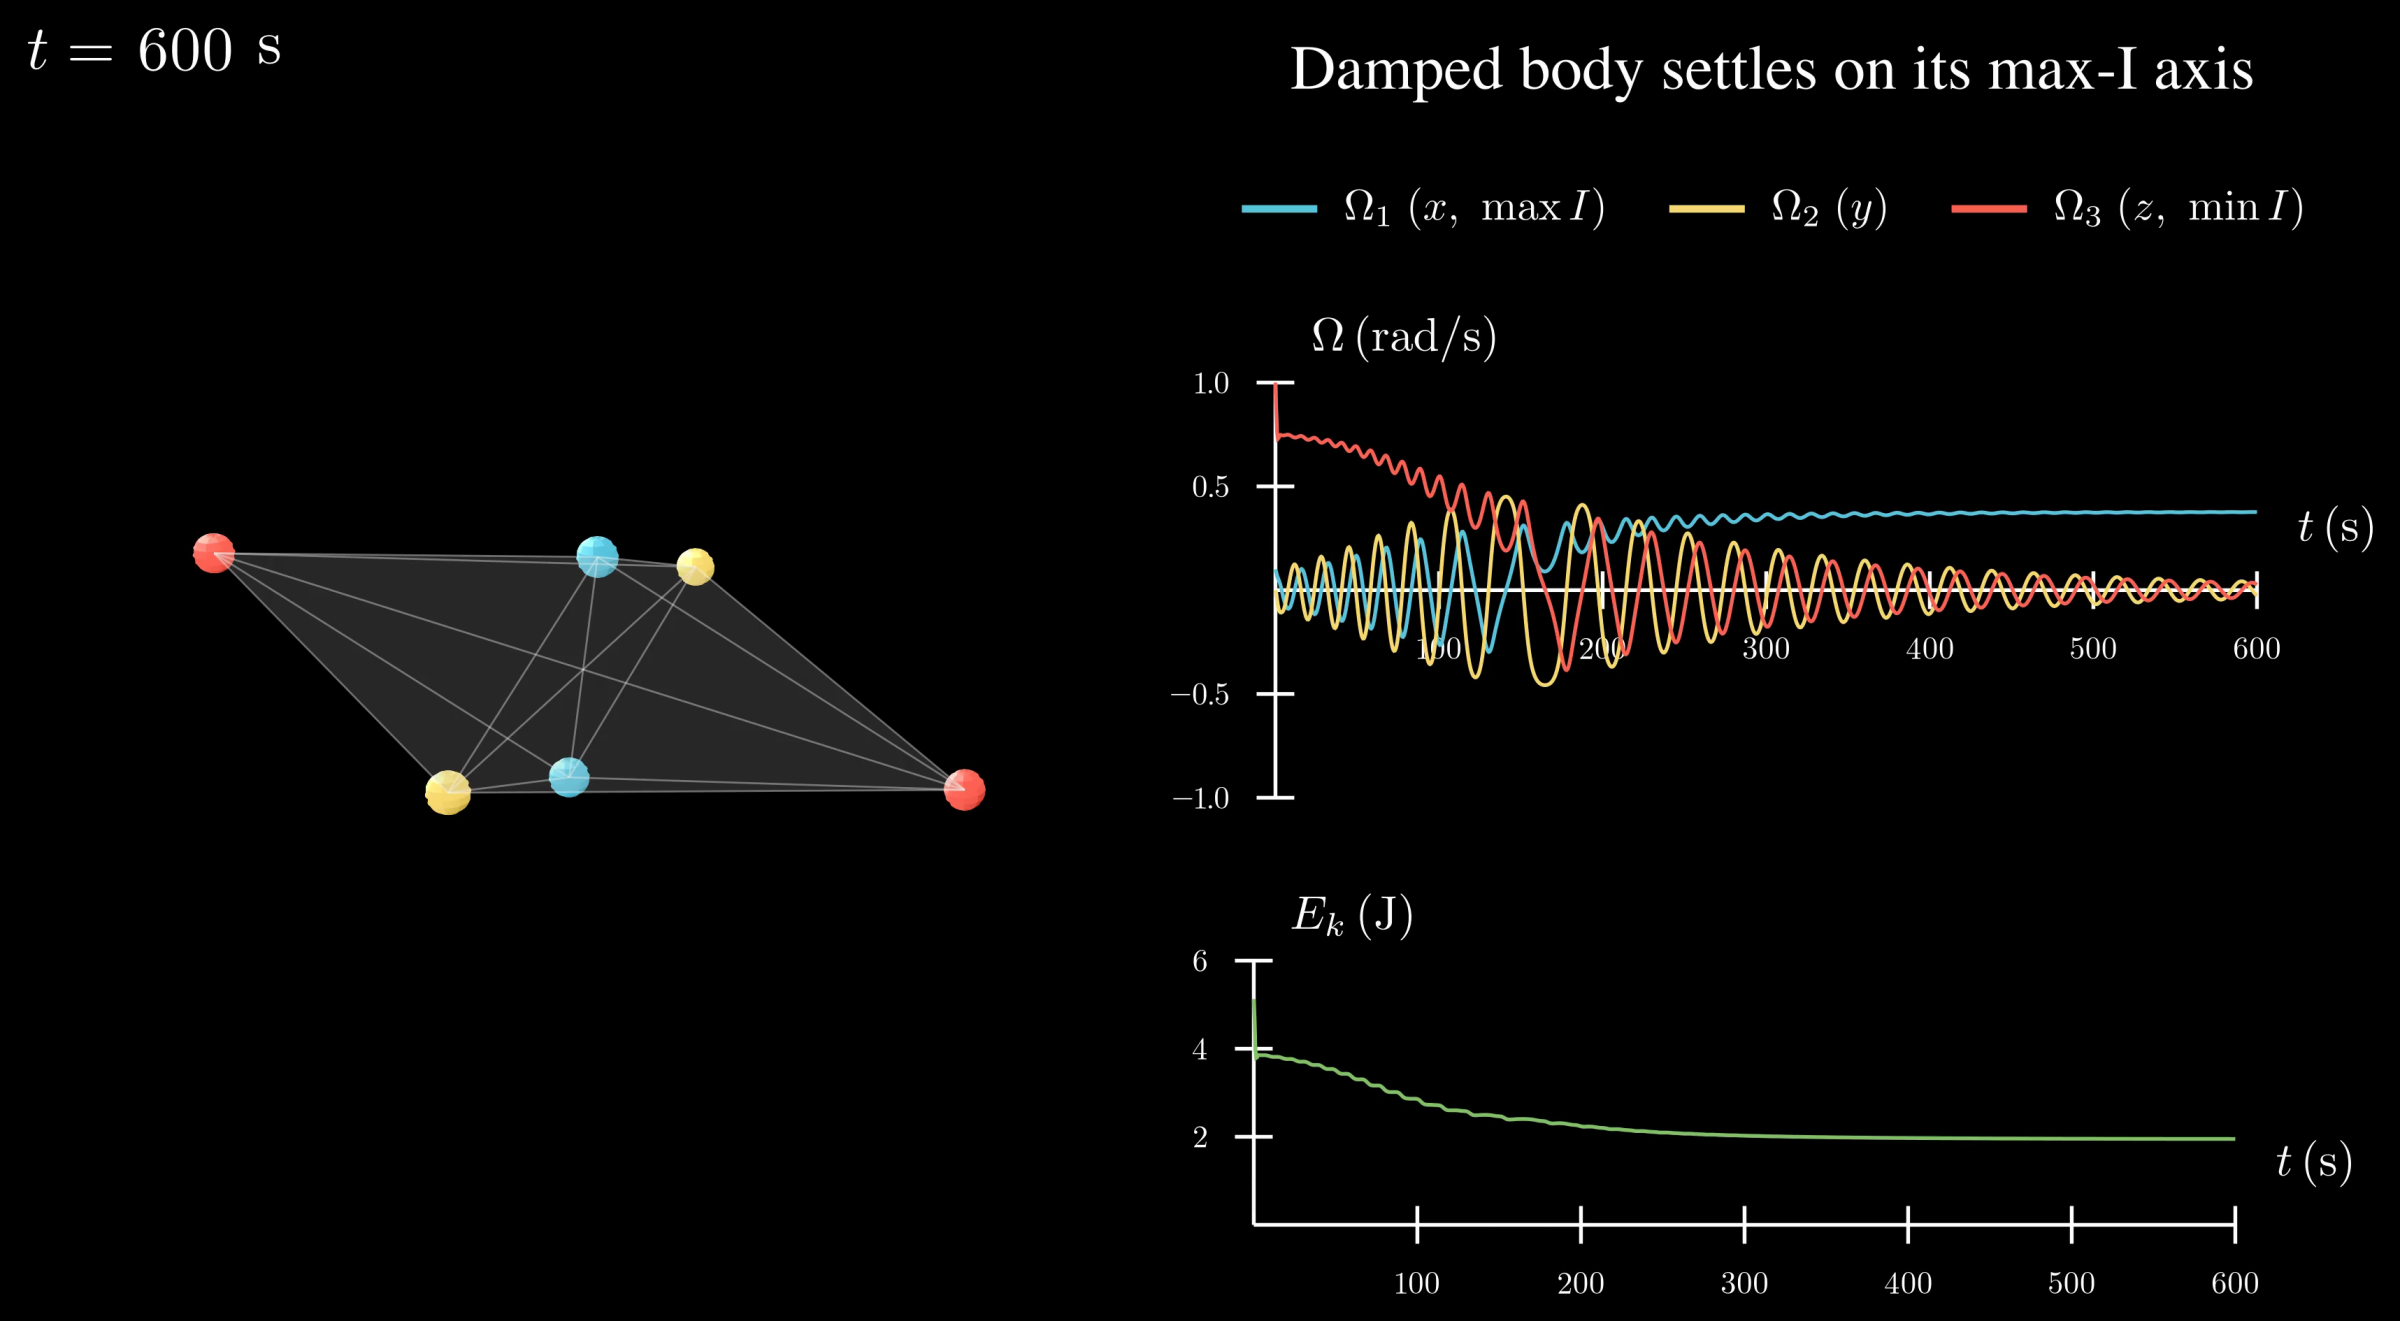
\includegraphics[width=0.8\textwidth]{Images/vis_major_axis.png}
    \caption{A damped body (soft springs, $k=\SI{1}{N/m}$, $c=\SI{0.7}{N.s/m}$) started spinning about its \emph{minor} axis $z$, slightly tilted toward $x$, shown at $t=\SI{600}{s}$. Top right: the spin about $z$ ($\Omega_3$) dies away while the spin about $x$, the major axis, grows and settles. Bottom right: the kinetic energy falls and levels off near $L^2/2I_{\max}\approx\SI{2.0}{J}$, the lowest energy possible at fixed $\vb{L}$ (\cref{sec:res-major}). Even rotation about the minor axis, stable for a rigid body, is not stable once the body can lose energy.}
    \label{fig:vis-major}
\end{figure*}

\section{Extension: energy loss in a non-rigid body}
\label{sec:extension}
So far the body has been almost perfectly rigid, and its energy has been conserved.
A real body is not perfectly rigid: it flexes slightly as it spins, and internal friction turns some of the energy of this wobbling into heat.
As an extension of the project we study what this energy loss does to the rotation.

\paragraph{The major axis rule}
No external torque acts, so $\vb{L}$ is still exactly conserved and only the energy $E$ decreases.
For a fixed $L$, the energy of rotation about a principal axis is $E=L^2/2I$, which is smallest for the largest $I$.
A body that keeps losing energy at fixed $L$ must therefore end up spinning about its major axis, whatever axis it started on.
This means that for a real, slightly flexible body only the major axis is truly stable: even spin about the minor axis, which is stable for a rigid body (\cref{sec:stability}), slowly drifts away.
This is what happened to Explorer 1 in 1958, and it is why the Earth, which spins about its major axis, keeps a steady rotation.

\paragraph{Model}
The spring model can show this directly, because its body is not perfectly rigid.
We give every spring a damping coefficient $c$, the second term in \cref{lst:spring}, which resists the two masses moving apart or together.
When the body turns rigidly the springs keep their length and the damping does nothing; only the wobbling is damped.
Like the spring force, the damping force is central and equal and opposite, so it removes energy but conserves momentum and angular momentum exactly.
This gives a useful check of the code: $\abs{\vb{L}}$ must stay constant while $E$ falls.

\begin{sloppypar} % units and symbols here would otherwise stick out of the column
We use soft springs, $k=\SI{1}{N/m}$, and $c=\SI{0.7}{N.s/m}$, so that the body wobbles noticeably and settles within a few hundred seconds, instead of the far longer time a nearly rigid body would take.
The soft springs also allow a larger time step, $\Delta t=\SI{5}{ms}$.
The octahedron starts spinning at \SI{1}{rad/s} about $z$, its minor axis, tilted slightly towards $x$, $\vb*{\omega}_0=(0.1,0,1)\,\si{rad/s}$, and is followed for \SI{1000}{s} with both engines.

\paragraph{Numerical details}
With a velocity-dependent force, velocity Verlet is no longer exactly symplectic, which is expected since the energy is meant to fall.
The damping force computed at the end of a step uses the velocity available at that point, the half-step velocity $\vb{v}^{n+1/2}$ (\cref{lst:verlet}).
This adds a small error, of relative size about $c\Delta t/m\approx0.004$ per step.
\end{sloppypar}

\paragraph{Expected outcome}
The initial angular momentum is $\vb{L}=(I_x\omega_x,0,I_z\omega_z)=(2.6,0,10)\,\si{kg.m^2/s}$, so $L\approx10.3\,\si{kg.m^2/s}$ and $E_0\approx\SI{5.1}{J}$.
If the body ends up spinning about $x$, it should turn at $\Omega_x=L/I_x\approx\SI{0.40}{rad/s}$ with $E=L^2/2I_x\approx\SI{2.05}{J}$.
These values are only approximate, because the soft springs let the body stretch and change its moments of inertia while it spins.
The run is shown in \cref{fig:vis-major} and analysed in \cref{sec:res-major}.

\section{Results}
\label{sec:results}
All results are for the octahedron of \cref{sec:inertia} simulated with the spring engines, unless stated otherwise.
The figures and numbers in this section come from \code{plot_results.py} and \code{plot_flip_time.py} in \code{src/sim/}.

\subsection{Stable rotation about the major and minor axes}
\label{sec:res-stable}
To compare the three axes directly, we spun the body at \SI{1}{rad/s} about each principal axis in turn, tilted by $\varepsilon=0.01$ toward the next axis, and followed it for \SI{100}{s} with the Python engine ($\Delta t=\SI{1}{ms}$, $k=\SI{e5}{N/m}$).
\Cref{fig:stable} shows the angle between the spin axis of the body and the fixed angular momentum.
About the axes of largest and smallest moment this angle only oscillates, between \ang{0.2} and \ang{0.44} about $x$ and between \ang{1.49} and \ang{1.65} about $z$, and does not grow over the whole run.
About the middle axis the same small tilt, initially \ang{0.29}, grows until the axis has turned over completely to \ang{180}, and then returns, about every \SI{48}{s}.

\begin{figure}[htb]
    \centering
    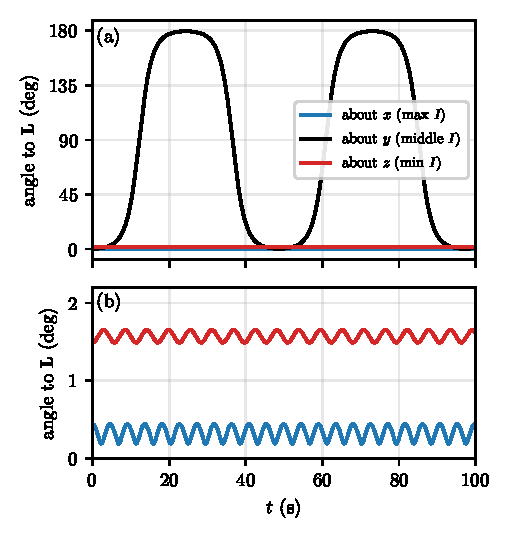
\includegraphics[width=\linewidth]{Images/stable_axes.pdf}
    \caption{Angle between the spin axis of the body and $\vb{L}$ for spins about each principal axis with the same small tilt. (a) All three runs: only rotation about the middle axis $y$ turns over. (b) Zoom on the runs about $x$ and $z$, where the angle stays bounded.}
    \label{fig:stable}
\end{figure}

\subsection{Rotation about the intermediate axis}
\label{sec:res-flip}
\begin{sloppypar} % long inline vector would otherwise stick out of the column
The main run spins the body about its middle axis with the Rust engine ($\Delta t=\SI{e-5}{s}$, $k=\SI{e5}{N/m}$, \SI{100}{s}); it is shown in \cref{fig:vis-omega,fig:vis-polhode}.
The body flips three times, each flip being a sign change of the component of $\vb{L}$ along the middle axis.
To test these times we solved Euler's equations (\cref{eq:euler}) for an ideal rigid body with SciPy's \code{solve_ivp} \cite{scipy} at a relative tolerance of $10^{-12}$, starting from the same angular velocity as the simulation, $\Omega_k=L_k(0)/I_k$, which gives $\vb*{\Omega}_0\approx(0.0015,1.0001,0)$\,\si{rad/s}.
The two agree to within one output frame, $\tfrac{1}{60}$\,s (\cref{tab:flips}), and the flips repeat every \SI{31.2}{s}.
Over the run the simulated $\vb{L}$ stays on the predicted polhode: $2E/L^2$ changes by less than $10^{-5}$ of its value, and $\abs{\vb{L}}$ by $1.4\times10^{-4}$, the latter mostly from the finite-difference velocities.
\end{sloppypar}

\begin{table}[htb]
    \centering
    \caption{Flip times for spin about the middle axis.}
    \label{tab:flips}
    \small
    \begin{tabular}{@{}lccc@{}}
        \toprule
                                      & 1st (s) & 2nd (s) & 3rd (s) \\
        \midrule
        Spring engine          & 15.60   & 46.82   & 78.03 \\
        Rigid body (Euler) & 15.61   & 46.82   & 78.03 \\
        \bottomrule
    \end{tabular}
\end{table}

\subsection{Flip time versus perturbation size}
\label{sec:res-fliptime}
\begin{sloppypar} % numbers with units would otherwise stick out of the column
\Cref{fig:flip-time} shows the time to the first flip for 500 initial tilts $\varepsilon$ between $2\times10^{-7}$ and $10^{-4}$, computed with the Rust engine ($\Delta t=\SI{1}{ms}$) for several spring stiffnesses, together with the rigid-body solution.
The flip time grows without bound as $\varepsilon\to0$, but only slowly: halving the tilt adds the same fixed amount of time.
Fitting $t_{\text{flip}}=\lambda^{-1}\ln(1/\varepsilon)+c$ to each set (\cref{tab:lambda}) confirms the logarithmic law of \cref{eq:tflip}; every fit has $R^2>0.9999996$.
For the stiffest springs the fitted growth rate, $\lambda=0.480383\pm0.000003\,\si{s^{-1}}$, matches the prediction of \cref{eq:lambda}, $\lambda=0.480384\,\si{s^{-1}}$, within its uncertainty.
Softer springs give a smaller $\lambda$ and later flips: the body stretches under its own rotation, which changes its moments of inertia.
\end{sloppypar}

\begin{figure}[htb]
    \centering
    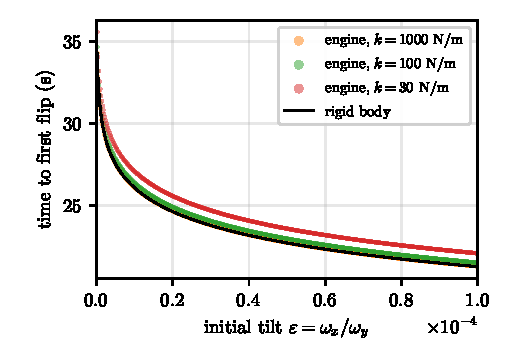
\includegraphics[width=\linewidth]{Images/flip_time.pdf}
    \caption{Time to the first flip against the initial tilt from the middle axis. Points: spring engine for three stiffnesses. Line: ideal rigid body from Euler's equations.}
    \label{fig:flip-time}
\end{figure}

\begin{table}[htb]
    \centering
    \caption{Growth rate $\lambda$ fitted to the flip times, compared with \cref{eq:lambda}.}
    \label{tab:lambda}
    \small
    \begin{tabular}{@{}lcc@{}}
        \toprule
        $k$ (N/m) & $\lambda$ (s$^{-1}$) & $\lambda/\lambda_{\text{theory}}$ \\
        \midrule
        $10^5$ & 0.48038 & 1.0000 \\
        $10^3$ & 0.47981 & 0.9988 \\
        $100$  & 0.47466 & 0.9881 \\
        $30$   & 0.46191 & 0.9615 \\
        \midrule
        Theory & 0.48038 & \\
        \bottomrule
    \end{tabular}
\end{table}

\subsection{Dissipation: relaxation to the major axis}
\label{sec:res-major}
The model and the expected outcome are described in \cref{sec:extension}; \cref{fig:dissipation} shows the damped run of the Rust engine.
At the start $\vb{L}$ is \ang{14.6} from the minimum axis $z$.
Over the first few hundred seconds the body wobbles away from $z$ and settles on the maximum axis $x$: by the end $\vb{L}$ is within \ang{0.7} of $x$.
Meanwhile $\abs{\vb{L}}$ stays constant to $5\times10^{-5}$, as it should for central damping forces.

\begin{sloppypar} % numbers with units would otherwise stick out of the column
The kinetic energy first drops quickly from \SI{5.13}{J} to about \SI{3.9}{J}, because the springs start at their rest length: the spinning body first expands, storing part of the energy in the springs, and the fast oscillation this starts is damped away at once.
After that it decays steadily and levels off at \SI{1.948}{J}.
This final value equals $L^2/2I_x=\SI{1.948}{J}$ when $I_x$ is computed from the actual, stretched shape of the body at the end ($I_x=\SI{27.4}{kg.m^2}$ instead of 26 at rest), so the body ends in steady rotation about $x$ at $\Omega_x=\SI{0.377}{rad/s}$.
The estimates of \cref{sec:extension}, \SI{2.05}{J} and \SI{0.40}{rad/s}, used the moment at rest, and the difference is exactly this stretching.
\end{sloppypar}

\begin{figure}[htb]
    \centering
    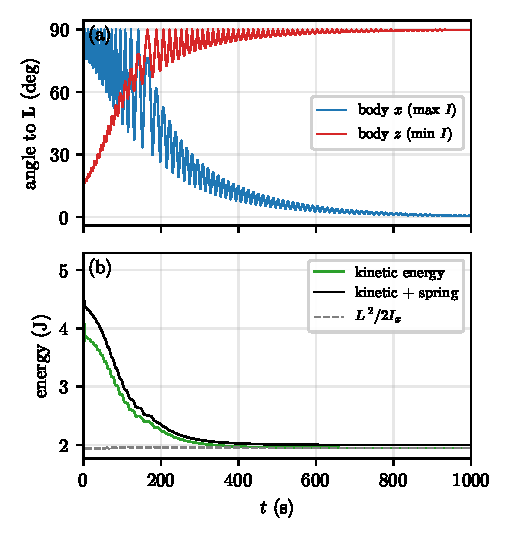
\includegraphics[width=\linewidth]{Images/dissipation.pdf}
    \caption{Damped body started near its minimum axis. (a) Angle between $\vb{L}$ and the body axes $x$ (max $I$) and $z$ (min $I$): the spin moves from $z$ to $x$. (b) Kinetic energy, kinetic plus spring energy, and the lowest energy possible at this $L$, $L^2/2I_x$, computed from the current shape of the body.}
    \label{fig:dissipation}
\end{figure}

\section{Validation and Error Analysis}
\label{sec:validation}
\begin{sloppypar}
The comparisons with the rigid body in \cref{sec:results} already test the spring model. Here we check the solvers themselves.
The numbers are computed by the script \code{plot_validation.py} in \code{src/sim/}.
\end{sloppypar}

\subsection{Exact solution}
\label{sec:analytic}
Euler's equations have an exact solution in Jacobi elliptic functions \cite{landau}.
The spin about the middle axis is proportional to $\operatorname{sn}$, which changes sign every half period, so the body flips every $T/2$ with
\begin{equation}
\begin{aligned}
    T &= 4K(k)\sqrt{\tfrac{I_1I_2I_3}{(I_3-I_2)(L^2-2EI_1)}},\\
    k^2 &= \tfrac{(I_2-I_1)(2EI_3-L^2)}{(I_3-I_2)(L^2-2EI_1)},
\end{aligned}
    \label{eq:jacobi-period}
\end{equation}
in Landau's labelling $I_1<I_2<I_3$, and $K$ the complete elliptic integral of the first kind.
\begin{sloppypar} % function names would otherwise stick out of the column
For the main run $1-k^2=4.9\times10^{-6}$; this close to the separatrix $1-k^2$ has to be computed directly, not as 1 minus $k^2$, or most of its digits are lost.
The solution, evaluated with \code{scipy.special.ellipj} and \code{ellipkm1} \cite{scipy}, gives flips every $T/2=\SI{31.213}{s}$, the same times as in \cref{tab:flips}.
The simulated $\vb*{\Omega}$ differs from it by a median of $2\times10^{-4}\,\si{rad/s}$, mostly from the finite-difference velocities.
\end{sloppypar}

\subsection{Conservation and convergence}
\label{sec:conservation}
\Cref{fig:conservation} follows the energy and angular momentum over \SI{100}{s}.
With velocity Verlet the energy error stays bounded, $2.5\times10^{-7}$ at $\Delta t=\SI{1}{ms}$ and four times smaller at half the step, and $\vb{L}$ is conserved to round-off, $3\times10^{-14}$, because the spring forces are central.
With RK4 the error is not bounded and builds up at each flip, but it is still only $8\times10^{-10}$ after \SI{100}{s} at $\Delta t=\SI{50}{ms}$.

\Cref{fig:convergence} confirms the order of both methods: $p=4.00$ for RK4 and $p\to2.00$ for Verlet.
Verlet only reaches its order once $\Delta t$ resolves the spring vibrations, 160--\SI{775}{rad/s}.
With the larger steps used in practice the phase of these vibrations is lost and the position error stays at a few $\si{\micro m}$, while the slow rotation that we measure stays accurate.

\begin{figure}[htb]
    \centering
    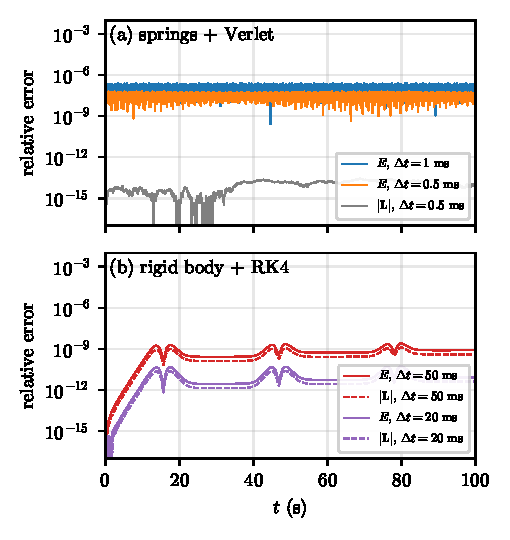
\includegraphics[width=\linewidth]{Images/conservation.pdf}
    \caption{Relative change of the energy and angular momentum. (a) Spring engine with Verlet. (b) Rigid-body solver with RK4.}
    \label{fig:conservation}
\end{figure}

\begin{figure}[htb]
    \centering
    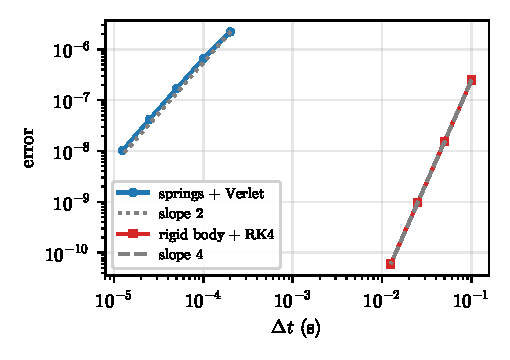
\includegraphics[width=\linewidth]{Images/convergence.pdf}
    \caption{Error against time step: Verlet (positions after \SI{1}{s}) and RK4 ($\vb*{\Omega}$ and $q$ after \SI{10}{s}), with slopes 2 and 4.}
    \label{fig:convergence}
\end{figure}

\subsection{Error budget}
\label{sec:error-budget}
The Python and Rust engines give bit-for-bit identical results after $10^5$ steps, and the stiffness error of the growth rate in \cref{tab:lambda} falls as about $(\SI{1.2}{N/m})/k$.
\Cref{tab:error-budget} collects the error sources for the main run.
The largest is not in the simulation but in the analysis, which reconstructs velocities from positions saved at \SI{60}{Hz}.

\begin{table}[htb]
    \centering
    \caption{Error sources for the main run ($\Delta t=\SI{e-5}{s}$, $k=\SI{e5}{N/m}$).}
    \label{tab:error-budget}
    \small
    \begin{tabular}{@{}lc@{}}
        \toprule
        Source & Relative size \\
        \midrule
        Time step (energy error)     & $\sim10^{-11}$ \\
        Finite stiffness ($\lambda$) & $\sim10^{-5}$ \\
        Velocities from \SI{60}{Hz} output & $\sim10^{-4}$ \\
        Floating point               & $\sim10^{-14}$ \\
        \bottomrule
    \end{tabular}
\end{table}

\section{Discussion}
\label{sec:discussion}
Both models reproduce the tennis racket effect.
In the spring model nothing about rigid bodies is coded, yet the flips appear from Newton's law for six point masses alone, at the times predicted by Euler's equations and the exact solution, and with the growth rate of the linear theory.
With damping added, the same model also shows the major axis rule.

The two models suit different jobs.
The spring model is general: any shape can be built from masses, and effects beyond a rigid body, such as flexing and internal friction, come for free.
Its cost is stiffness: the time step is set by spring vibrations several hundred times faster than the rotation, so the main run needed $10^7$ steps, and was only practical after moving from Python to Rust.
The rigid-body solver with quaternions has only seven variables and no fast motion, so a step of \SI{50}{ms} already keeps the energy to $10^{-9}$, but it can only describe a perfectly rigid body.
The main limitation of our analysis was not in either solver but in recovering velocities from positions saved at \SI{60}{Hz}, which sets the error floor of about $10^{-4}$.

\subsection{Extensions}
\label{sec:extensions}
\paragraph{Constraint solvers}
Instead of stiff springs, the distances between the masses can be held fixed as exact constraints.
SHAKE \cite{shake1977} and its velocity form RATTLE \cite{rattle1983} add Lagrange-multiplier forces to each Verlet step so that every bond length is restored exactly, while keeping Verlet's symplectic, time-reversible character \cite{hairer2006}.
This removes the fast vibrations, so the time step would be set by the rotation, as for the rigid-body solver, while keeping the generality of a particle model.
The price is a set of nonlinear constraint equations to solve iteratively at every step.

\paragraph{Chaos}
The free rigid body is integrable: with energy and $\abs{\vb{L}}$ conserved its motion is regular, and even near the separatrix the flips are periodic, with a flip time that grows only logarithmically as the tilt shrinks.
This changes once integrability is broken, for example by gravity acting on an asymmetric top, a periodic external torque, or a second body attached by a joint.
The separatrix then turns into a thin chaotic layer, and the flips occur at irregular times.
Such forces can be added to our engine without changing the integrator, and the chaos measured by the divergence of two runs started a tiny distance apart (a Lyapunov exponent).

\paragraph{Lie groups}
Orientations form the rotation group $SO(3)$, a Lie group, and unit quaternions form its double cover.
Our RK4 step moves $q$ off the unit sphere and projects it back by normalising, so it neither stays on the group nor preserves the structure of the equations, which is why its energy error accumulates (\cref{fig:conservation}).
Lie-group integrators instead update the orientation with the exponential map, $q_{n+1}=q_n\otimes\exp\!\big(\tfrac12\vb*{\Omega}\Delta t\big)$, which stays on the group exactly.
Splitting the free rigid body into rotations about its three axes, each of which can be solved exactly, gives symplectic methods that conserve $\abs{\vb{L}}$ exactly and keep the energy error bounded \cite{hairer2006}, the same advantage Verlet gives the spring model.

%\clearpage                                     % Sometimes you want the rest on separate pages.
\section*{Use of AI tools}
AI tools were used in the initial drafts of this report. We also used AI to make all the beautiful videos using Manim as already mentioned above.
We used it to make some of the plots shown in results and validation. All the code pertaining to the actual physics engine and everything before calling the function to generate the CSV file is done by us.
We consider this as fair use.
                   % Use of AI tools

%%%%%%%%%%%%%%%%%%%%%%%%%%%%%%%%%%%%%%%%

% Bibliography
%--------------------
\printbibliography

%\clearpage                                     % Sometimes it is useful to have appendix on separate page.
%\onecolumn                                     % If you want 1 column for appendix.
\appendix

\section{Supplementary videos}
\label{app:videos}
The videos are in the \href{\repourl/tree/main/videos}{\code{videos/}} folder of the project repository.
\begin{table}[H]
    \centering
    \caption{Supplementary Manim videos.}
    \label{tab:videos}
    \small
    \begin{tabularx}{\columnwidth}{@{}l L l@{}}
        \toprule
        Video & Content & File \\
        \midrule
        V1 & Octahedron spun about its middle axis, with live $\Omega_k(t)$ & \href{\repourl/blob/main/videos/spin_middle_axis.mp4}{link} \\
        V2 & Same run: the body with the fixed $\vb{L}$, and $\vb{L}$ on the sphere and energy ellipsoid & \href{\repourl/blob/main/videos/polhode.mp4}{link} \\
        V3 & Damped body settling on its major axis & \href{\repourl/blob/main/videos/major_axis.mp4}{link} \\
        V4 & Tennis racket toss, quaternion solver & \href{\repourl/blob/main/videos/racket_toss.mp4}{link} \\
        \bottomrule
    \end{tabularx}
\end{table}
                           % Comment out to exclude appendix

\end{document}

% Template: "NTNU Laboratory Report in Physics" by Vebjørn S. Førde, CC BY 4.0
% https://www.overleaf.com/latex/templates/ntnu-laboratory-report-in-physics/zrkxstqtpdpv
% Changes: extra packages and helper macros above, Validation section and content in Text/.
